\documentclass[tikz]{standalone}
\renewcommand*{\familydefault}{\sfdefault}
\usepackage{standalone}
\usepackage{amssymb}
\usetikzlibrary{decorations}
%\usetikzlibrary{arrows.meta, decorations.pathmorphing, decorations.pathreplacing, shapes.geometric}
\usetikzlibrary{bayesnet}

\begin{document}
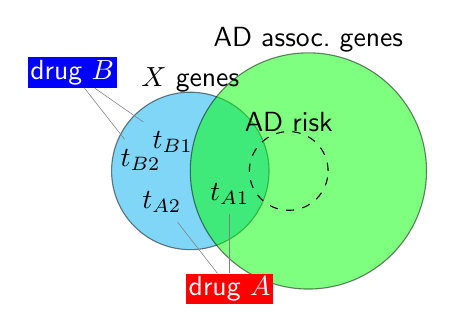
\begin{tikzpicture}[pin distance=0.75cm]%[font=\footnotesize, xscale=1.5]
\draw[draw,fill=cyan,semitransparent] (0.5,0) circle(1.0);
\draw[draw,fill=green,semitransparent] (2.,0) circle(1.5);
\draw[draw,dashed] (1.75,0) circle(0.5);
%\draw (0,0) circle(3) (4,0) circle(4);
\path (1,-1.5) node[white,rectangle,inner sep=1pt,fill=red,
	pin=90:$t_{A1}$,
	pin=120:$t_{A2}$] {drug $A$};
\path (-1.0,1.25) node[white,rectangle,inner sep=1pt,fill=blue,
	pin=-35:$t_{B1}$,
	pin=-60:$t_{B2}$] {drug $B$};
\node[anchor=south,inner sep=0pt] (X) at (0.5,1.0) {$X$ genes};
\node[anchor=south,inner sep=0pt] (X) at (2.0,1.5) {AD assoc.~genes};
\node[anchor=south,inner sep=0pt] (X) at (1.75,0.5) {AD risk};
\end{tikzpicture}
\end{document}
